\documentclass[conference,a4paper]{IEEEtran}
\usepackage[utf8]{inputenc}
\usepackage[T1]{fontenc}
\usepackage{amsmath,amssymb,graphicx,booktabs,cite,url}
\usepackage[hidelinks]{hyperref}
% Auteurs et enseignant.
\newcommand{\AuteurUn}{Abderrahman Boubligha}
\newcommand{\AuteurDeux}{Mohamed Reda Lakouas}
\newcommand{\Enseignant}{Aissam Hadri}

\renewcommand{\abstractname}{Résumé}
\renewcommand{\IEEEkeywordsname}{Mots-clés}
\renewcommand{\refname}{Références}
\title{Régression linéaire et prix des logements :\\étude comparative de méthodes d'optimisation}
\author{\IEEEauthorblockN{\AuteurUn\ et\ \AuteurDeux}
\IEEEauthorblockA{Master 1 -- Optimisation numérique\\Projet SAM -- Année universitaire 2026--2027\\Enseignant : \Enseignant}}
\begin{document}
\maketitle
\begin{abstract}
Ce travail étudie l'optimisation par essaim particulaire pour calculer les coefficients d'une régression linéaire appliquée au prix des logements. Les données réelles comprennent 414 observations de New Taipei, à Taiwan. Le modèle utilise six variables et prédit un prix par unité de surface. Nous comparons quatre méthodes de calcul des coefficients : essaim particulaire, descente de gradient, recherche aléatoire et moindres carrés. Une prédiction constante sert aussi de référence simple. Le partage principal utilise 331 observations pour apprendre et 83 pour tester. Les deux méthodes aléatoires sont répétées avec vingt initialisations. L'essaim particulaire, la descente de gradient et les moindres carrés donnent une erreur quadratique moyenne sous sa forme racine d'environ 8,21 et un coefficient de détermination de 0,5632 sur le test. La recherche aléatoire est moins précise au même budget d'évaluations que l'essaim. Des expériences supplémentaires étudient la taille de l'essaim, les résidus et cinq autres partages. Les résultats montrent surtout que la stabilité de l'optimisation ne garantit pas une bonne précision sur tous les logements. Les conclusions restent limitées à une petite base historique et à un modèle linéaire.
\end{abstract}
\begin{IEEEkeywords}optimisation par essaim particulaire, régression linéaire, descente de gradient, prix immobilier, comparaison expérimentale.\end{IEEEkeywords}

\section{Introduction}
Le prix d'un logement dépend de sa localisation, de son âge et de son environnement. Un modèle de régression cherche une relation entre ces informations et un prix observé. Ce problème permet d'étudier à la fois la prédiction et l'optimisation numérique : avant de prédire, il faut trouver les paramètres du modèle.

Dans ce projet, le modèle est une régression linéaire. La méthode principale est l'optimisation par essaim particulaire, appelée PSO. Chaque particule représente une solution possible. Elle se déplace en utilisant sa mémoire et la meilleure solution du groupe. Le principe a été présenté par Kennedy et Eberhart \cite{kennedy}. Il permet de chercher une solution sans calculer de dérivée de l'objectif.

Une difficulté importante est de bien séparer deux questions. La première est : \textit{l'algorithme trouve-t-il les bons coefficients pour l'objectif choisi ?} La seconde est : \textit{le modèle prédit-il correctement les prix de logements non utilisés pour apprendre ?} Un algorithme peut résoudre très précisément le problème d'apprentissage et conserver des erreurs de prédiction importantes.

Notre étude répond à trois questions :
\begin{enumerate}
\item Le PSO retrouve-t-il une solution proche des moindres carrés et de la descente de gradient ?
\item Apporte-t-il un avantage sur une recherche aléatoire sans mémoire, au même nombre d'évaluations ?
\item Les résultats changent-ils avec l'initialisation, le budget ou le partage des données ?
\end{enumerate}
Nous utilisons une base réelle et conservons une implémentation lisible. Le travail comprend une analyse descriptive, une formulation mathématique, des comparaisons répétées, une analyse des erreurs et une petite application. Il ne propose pas un nouvel algorithme et ne prétend pas dépasser les méthodes classiques sur tous les problèmes.

\section{Travaux liés et positionnement}
\subsection{Estimation immobilière}
La base Real Estate Valuation est distribuée par le dépôt UCI \cite{uci}. L'article associé de Yeh et Hsu étudie une approche comparative de l'estimation immobilière \cite{yeh}. Nous utilisons les données comme support expérimental, mais nous ne reproduisons pas leur méthode ni leurs résultats. Le partage et les algorithmes employés ici sont décrits séparément pour éviter une comparaison directe injustifiée.

Une régression linéaire est intéressante pour un premier projet : elle contient peu de paramètres et son objectif peut être écrit explicitement. Elle ne décrit toutefois pas toutes les relations possibles. La distance à un transport peut avoir un effet qui n'est pas proportionnel à chaque mètre. Des logements proches peuvent aussi partager des caractéristiques absentes de la base.
\subsection{Méthodes d'optimisation}
Le PSO repose sur l'échange d'information dans un essaim \cite{kennedy}. Shi et Eberhart ont étudié l'ajout d'un poids d'inertie \cite{shi}. Notre version utilise une inertie qui diminue de 0,9 à 0,4. Il s'agit d'un choix pratique de cette implémentation ; nous ne prétendons pas reproduire exactement une variante publiée.

Les méthodes de gradient exploitent au contraire la dérivée de l'objectif. Le cadre de l'optimisation convexe explique pourquoi un minimum fiable peut être obtenu pour une régression linéaire aux moindres carrés \cite{boyd}. Cette propriété fournit une référence utile pour vérifier le PSO.

La recherche aléatoire est une comparaison simple : elle essaie des solutions indépendantes et conserve la meilleure. Bergstra et Bengio discutent son intérêt comme référence pour la recherche d'hyperparamètres \cite{bergstra}. Ici, nous appliquons ce principe directement aux coefficients du modèle, et non aux hyperparamètres. Le domaine, le nombre de candidats et l'objectif sont donc propres à notre expérience.

\section{Données et analyse descriptive}
\subsection{Source, contrôle et unités}
Le fichier Excel fourni contient 414 lignes et huit colonnes : un identifiant, six variables et une cible. Les observations concernent New Taipei, à Taiwan, avec des dates de transaction entre 2012 et 2013. La base est réutilisée sous licence CC BY 4.0 avec mention de sa source \cite{uci}.

Nous avons vérifié que les valeurs sont numériques et finies. Aucune valeur manquante ni ligne dupliquée hors identifiant n'a été trouvée. Nous conservons toutes les lignes, y compris celles dont le prix est élevé. Le fichier CSV garde les valeurs numériques du fichier Excel, avec des en-têtes plus courts. La colonne \texttt{No} est exclue du modèle : elle identifie une ligne, mais ne décrit pas un logement.

La cible est un prix par unité de surface, en \textbf{10\,000 dollars de Taiwan par ping}. Un ping vaut environ 3,3 m$^2$ selon la documentation UCI. Par exemple, une valeur de 40 correspond à 400\,000 dollars de Taiwan par ping. Elle n'est ni le prix total du logement ni un montant en dirhams marocains.
\begin{table}[t]
\caption{Variables disponibles et rôle dans l'étude.}
\label{tab:variables}\centering\small
\begin{tabular}{lll}\toprule
Colonne & Information & Unité\\\midrule
$X_1$ & Date de transaction & année décimale\\
$X_2$ & Âge du logement & années\\
$X_3$ & Distance au métro & mètres\\
$X_4$ & Commerces proches & nombre\\
$X_5$ & Latitude & degrés\\
$X_6$ & Longitude & degrés\\
$Y$ & Prix par surface & $10^4$ TWD/ping\\\bottomrule
\end{tabular}
\end{table}
Le tableau~\ref{tab:variables} présente les six entrées. La date suit la convention fournie par la source : 2013,5 représente juin 2013. La base ne contient ni la surface totale du logement, ni son nombre de chambres. Ces informations ne sont donc pas inventées dans l'application.

\subsection{Distribution des observations}
La figure~\ref{fig:distribution} montre la distribution des prix et des distances au métro. Elle sert à repérer les zones les plus représentées et les observations éloignées du reste. Le prix varie de 7,6 à 117,5 et l'âge de 0 à 43,8 ans. Les distances vont d'environ 23 à 6\,488 mètres. Le nombre de commerces varie de 0 à 10.
\begin{figure*}[t]\centering
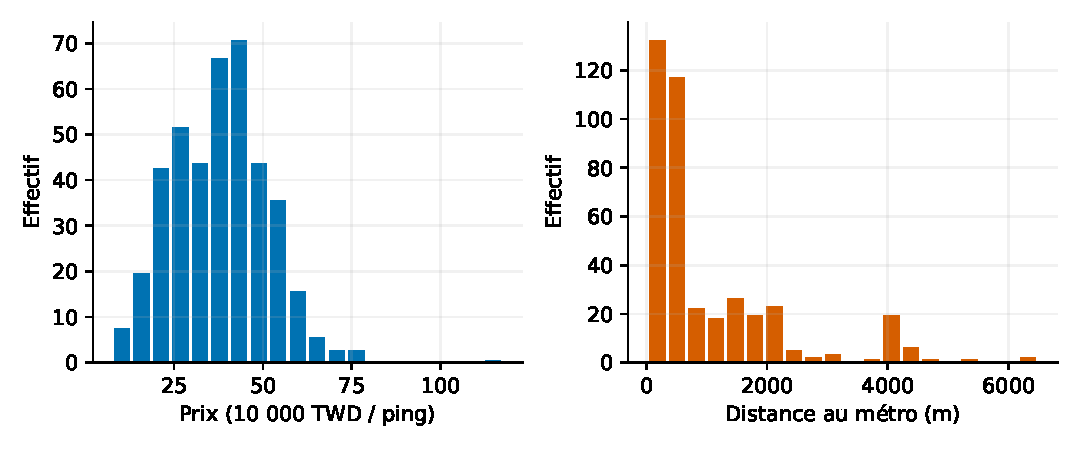
\includegraphics[width=.92\textwidth]{figures/distribution.pdf}
\caption{Distribution des 414 prix observés et des distances au métro. Les prix sont en $10^4$ TWD par ping. Ces graphiques décrivent toute la base et ne servent pas à régler les algorithmes.}\label{fig:distribution}
\end{figure*}
Une distribution concentrée avec quelques valeurs élevées peut rendre la RMSE sensible à un petit nombre de grandes erreurs. Cela justifie l'emploi de plusieurs indicateurs et l'examen des résidus, plutôt qu'un seul score global. Nous ne retirons pas les observations extrêmes après avoir regardé leur effet sur le test.

\subsection{Corrélations et localisation}
La matrice de la figure~\ref{fig:correlations} contient les corrélations de Pearson calculées sur toute la base. Elle décrit des associations linéaires entre les colonnes. Une corrélation proche de zéro ne prouve pas l'absence de relation non linéaire. Une corrélation élevée ne démontre pas non plus une cause.
\begin{figure}[t]\centering
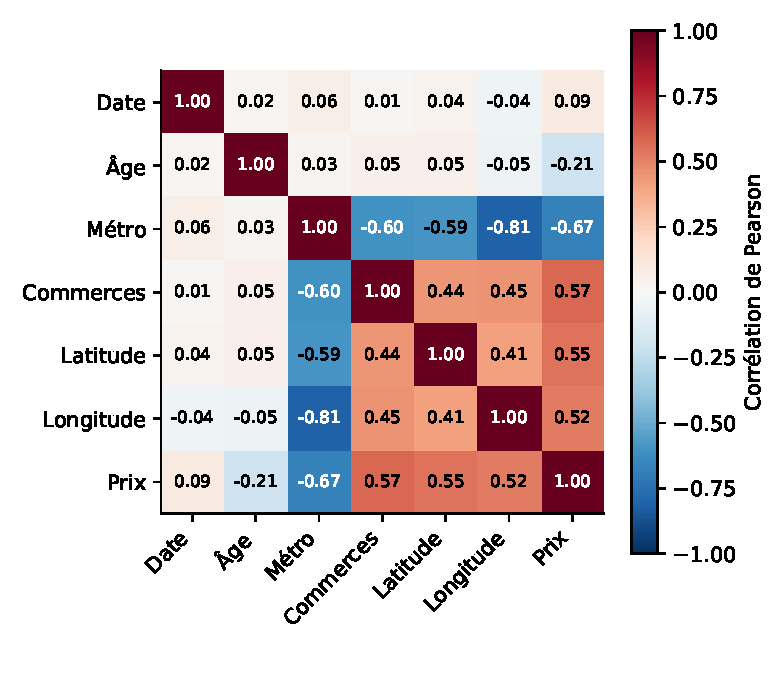
\includegraphics[width=\columnwidth]{figures/correlations.pdf}
\caption{Corrélations descriptives. Le rouge indique une association positive et le bleu une association négative. Les valeurs restent lisibles sans se limiter à la couleur.}\label{fig:correlations}
\end{figure}
Les relations entre les variables explicatives sont importantes : si plusieurs colonnes apportent une information proche, les coefficients individuels peuvent être difficiles à interpréter. Pour cette raison, nous ne présentons pas les poids de la régression comme des effets économiques certains.

La figure~\ref{fig:geo} situe les observations avec leur longitude et leur latitude, et représente le prix par la couleur. Il ne s'agit pas d'une carte avec un fond géographique. Le graphique permet surtout de voir la concentration spatiale de l'échantillon. Deux logements proches peuvent se retrouver de part et d'autre d'un partage aléatoire ; nous reviendrons sur cette limite.
\begin{figure}[t]\centering
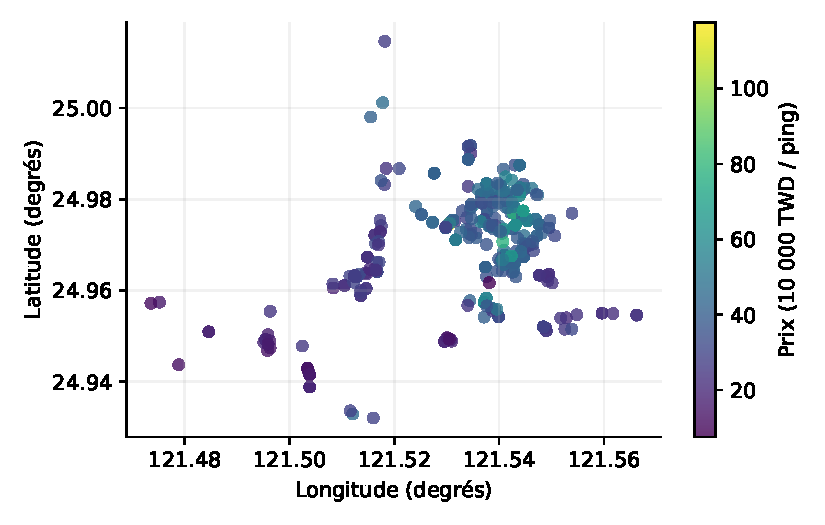
\includegraphics[width=\columnwidth]{figures/geographie.pdf}
\caption{Positions des observations et prix par unité de surface. La couleur représente le prix historique, sans interpolation entre les points.}\label{fig:geo}
\end{figure}

\section{Formulation du modèle}
\subsection{Prédiction et fonction objectif}
Pour une observation $i$, la régression linéaire calcule
\begin{equation}
\widehat y_i=\beta_0+\sum_{j=1}^{6}\beta_jx_{ij}.
\end{equation}
Il y a sept paramètres : une constante et six coefficients. Le modèle associe chaque variable à un poids. La prédiction est un prix par surface. Il s'agit du même modèle pour tous les optimiseurs comparés.

Pour mesurer l'ajustement sur l'apprentissage, nous utilisons l'erreur quadratique moyenne :
\begin{equation}
J(\theta)=\frac{1}{n}\sum_{i=1}^{n}(u_i-\widehat u_i)^2
=\frac{1}{n}\|A\theta-u\|_2^2.
\label{eq:objectif}
\end{equation}
Ici, $n=331$, $u$ est le prix standardisé et $A$ contient les six variables standardisées et une première colonne de 1. Le vecteur $\theta$ contient les coefficients dans cette nouvelle échelle. Une petite valeur de $J$ signifie que les prédictions sont proches des observations d'apprentissage. Elle ne suffit pas pour conclure sur des logements nouveaux.

\subsection{Standardisation sans fuite du test}
Chaque variable est transformée par
\begin{equation}
z_j=\frac{x_j-\mu_j}{\sigma_j},\qquad
u=\frac{y-\mu_y}{\sigma_y}.
\end{equation}
Les moyennes et écarts-types sont calculés seulement sur les lignes d'apprentissage. Nous réutilisons exactement ces valeurs pour transformer le test. Cela évite d'ajuster une transformation avec des informations provenant du test.

La standardisation rapproche les échelles : quelques unités pour les commerces, plusieurs milliers pour la distance et de petites variations pour les coordonnées. Elle rend les bornes de recherche plus faciles à définir. Les coefficients cherchés par le PSO sont limités à $[-5,5]$. Cette borne n'est pas une loi immobilière : c'est une contrainte numérique de l'expérience.

Pour retrouver le prix original, on multiplie la prédiction standardisée par $\sigma_y$ puis on ajoute $\mu_y$. Les poids dans les unités de départ sont calculés par
\begin{equation}
\beta_j=\frac{\sigma_y}{\sigma_j}\theta_j,\quad
\beta_0=\mu_y+\sigma_y\theta_0-\sum_{j=1}^{6}\beta_j\mu_j.
\end{equation}
Le modèle sauvegardé utilise ces coefficients. L'application peut donc effectuer une simple somme de produits sans refaire les transformations.

\subsection{Pourquoi les moindres carrés sont une référence}
La fonction de l'équation~\eqref{eq:objectif} est quadratique et convexe. Sa hessienne vaut $2A^TA/n$ et ne contient pas de direction de courbure négative \cite{boyd}. Le problème est ainsi différent d'un problème général avec de nombreux minima locaux.

Nous obtenons la solution de référence avec \texttt{numpy.linalg.lstsq} \cite{lstsq}. Il n'est pas nécessaire de calculer explicitement l'inverse de $A^TA$. Le code vérifie que les coefficients de cette solution restent à l'intérieur des bornes du PSO pour le partage principal. La comparaison entre objectif contraint et référence non contrainte est donc cohérente dans cette expérience.

\section{Algorithmes comparés}
\subsection{Optimisation par essaim particulaire}
Chaque particule $k$ possède une position $q_k$, une vitesse $v_k$, sa meilleure position personnelle $p_k$ et la meilleure position globale $g$. Sa position comporte sept nombres. Elle ne représente pas une observation de la base.

À chaque itération, la mise à jour est
\begin{align}
v_k^{t+1}&=w_tv_k^t+1{,}5r_1\odot(p_k-q_k^t)\notag\\
&\quad+1{,}5r_2\odot(g-q_k^t),\\
q_k^{t+1}&=\Pi_{[-5,5]^7}(q_k^t+v_k^{t+1}).
\end{align}
Les vecteurs $r_1$ et $r_2$ sont tirés uniformément entre 0 et 1, séparément pour chaque particule et coordonnée. Le premier terme conserve une partie du mouvement, le deuxième utilise la mémoire personnelle et le troisième exploite la meilleure solution du groupe.

Le poids $w_t$ diminue de 0,9 à 0,4 pendant 400 itérations. Les vitesses commencent à zéro et restent entre $-1$ et $1$. Une coordonnée dépassant une borne est ramenée à cette borne ; sa vitesse est alors mise à zéro. Les positions initiales sont uniformes dans le domaine de recherche. Nous utilisons 40 particules dans l'expérience principale.
\begin{table}[t]\centering\small
\caption{Déroulement d'une exécution du PSO.}\label{tab:pseudo}
\begin{tabular}{p{.94\columnwidth}}\toprule
1. Créer les 40 positions et les vitesses nulles.\\
2. Calculer les coûts et initialiser les meilleurs résultats.\\
3. Pour chaque itération, conserver le meilleur global courant.\\
4. Pour chaque particule : calculer la vitesse, déplacer la position et appliquer les bornes.\\
5. Mettre à jour les meilleurs personnels puis le meilleur global.\\
6. Sauvegarder le meilleur coût et répéter jusqu'à 400 itérations.\\
7. Retourner les sept coefficients de la meilleure position.\\\bottomrule
\end{tabular}
\end{table}
Le tableau~\ref{tab:pseudo} donne les étapes du code. La conservation du meilleur résultat produit une courbe non croissante. Cela ne prouve pas, à elle seule, que le minimum global est atteint. La proximité avec les moindres carrés est un contrôle supplémentaire propre à ce problème.

\subsection{Descente de gradient}
La descente de gradient modifie directement un seul vecteur de coefficients :
\begin{align}
\nabla J(\theta)&=\frac{2}{n}A^T(A\theta-u),\\
\theta^{t+1}&=\Pi_{[-5,5]^7}(\theta^t-\eta\nabla J(\theta^t)).
\end{align}
Les coefficients commencent à zéro. Le pas $\eta$ est l'inverse de la plus grande valeur propre de la hessienne. Il est donc calculé sur l'apprentissage, sans utiliser le test. Pour le partage principal, il vaut environ 0,1846. Ce choix évite une recherche de pas basée sur les résultats de test \cite{boyd}.

Nous effectuons 400 mises à jour. La projection maintient les mêmes bornes que le PSO. La méthode exploite la dérivée, contrairement au PSO et à la recherche aléatoire. Une itération de gradient n'a donc ni le même contenu ni le même coût qu'une itération d'essaim.

\subsection{Recherche aléatoire et prédiction constante}
La recherche aléatoire tire des vecteurs indépendants uniformément dans $[-5,5]^7$, calcule leur coût et conserve le meilleur. Elle n'utilise ni vitesse, ni mémoire personnelle, ni attraction collective. Elle permet de vérifier si le déplacement organisé de l'essaim apporte un avantage par rapport à de simples essais.

Nous lui donnons 16\,040 candidats, soit le même nombre d'évaluations de coût que le PSO : 40 positions initiales et $40\times400$ nouvelles positions. Le code regroupe les candidats par 40 pour enregistrer une courbe comparable, mais les tirages restent indépendants.

Enfin, une prédiction constante égale à la moyenne des prix d'apprentissage sert de seuil de comparaison. Une méthode qui ne fait pas mieux que cette valeur doit être examinée avec prudence. Cette référence ne recherche pas les coefficients d'un modèle à six variables.

\section{Protocole expérimental}
\subsection{Séparation et paramètres fixés}
Le partage principal utilise une permutation aléatoire de graine 42 : les 331 premières lignes servent à apprendre et les 83 autres à tester. Il ne reproduit pas le partage deux tiers/un tiers mentionné par la page UCI. Toutes les méthodes utilisent exactement les mêmes lignes et les mêmes transformations.

Les paramètres du PSO principal ont été conservés depuis la première version du projet, avant l'emploi de ces données réelles. Le test ne participe jamais au coût ni au déplacement des particules. Nous n'avons pas choisi le meilleur algorithme ou la meilleure taille d'essaim selon le score de test.
\begin{table}[t]\centering\small
\caption{Expériences réalisées et information utilisée.}\label{tab:protocole}
\begin{tabular}{p{.25\columnwidth}p{.65\columnwidth}}\toprule
Expérience & Réglage et rôle\\\midrule
Comparaison & Partage 42 ; 20 graines pour PSO et recherche aléatoire.\\
Gradient & 400 mises à jour ; pas calculé sur l'apprentissage.\\
Sensibilité & 10, 20, 40, 80 particules ; 10 graines ; budget court de 1\,600 coûts ; apprentissage seulement.\\
Autres partages & Graines 10, 20, 30, 40, 50 ; 331/83 lignes ; PSO de graine 0 et OLS.\\\bottomrule
\end{tabular}
\end{table}
Le tableau~\ref{tab:protocole} distingue les expériences. Les 20 initialisations du partage principal mesurent la variabilité de l'optimiseur, pas celle de l'échantillonnage. Les cinq autres partages étudient une autre source de variation : le choix des logements de test.

\subsection{Mesures et coût de calcul}
Les prédictions sont remises dans l'unité originale avant l'évaluation. Avec $m=83$ et $e_i=y_i-\widehat y_i$, nous calculons
\begin{align}
\mathrm{RMSE}&=\sqrt{\frac{1}{m}\sum_i e_i^2},\\
\mathrm{MAE}&=\frac{1}{m}\sum_i|e_i|,\\
R^2&=1-\frac{\sum_i e_i^2}{\sum_i(y_i-\overline y_{\rm test})^2}.
\end{align}
RMSE et MAE s'expriment en $10^4$ TWD par ping. La RMSE donne davantage de poids aux grosses erreurs. Le coefficient $R^2$ peut être négatif et ne représente pas un pourcentage de prédictions exactes \cite{r2}.

Nous enregistrons aussi le coût d'apprentissage standardisé et la durée d'ajustement. Les durées excluent la lecture des fichiers, le tracé et l'évaluation sur le test. La descente de gradient inclut le calcul de son pas. OLS et gradient sont répétés 20 fois pour mesurer la durée ; leurs résultats ne changent pas car ils sont déterministes dans cette configuration.

L'égalité des 16\,040 évaluations concerne seulement PSO et recherche aléatoire. Elle ne permet pas de comparer directement tous les algorithmes en nombre d'itérations. Les temps dépendent des boucles Python, du matériel et des bibliothèques. Ils décrivent cette implémentation, pas une vitesse universelle.

\section{Résultats et analyse}
\subsection{Qualité prédictive et temps}
\begin{table*}[t]\centering\small
\caption{Comparaison sur le partage principal : moyennes et écarts-types de 20 exécutions. Erreurs en $10^4$ TWD par ping. OLS, gradient et moyenne sont déterministes ; leurs répétitions servent au chronométrage.}
\label{tab:resultats}
\begin{tabular}{lrrrrr}\toprule
Méthode & RMSE & Écart-type RMSE & MAE & $R^2$ & Temps moyen (ms)\\\midrule
Moyenne & 12,4216 & 0 & 9,5698 & -0,0000 & 0,000\\
Recherche aléatoire & 23,5020 & 3,6343 & 18,5251 & -2,6612 & 124,537\\
Gradient & 8,2099 & 0 & 6,1620 & 0,5632 & 6,314\\
PSO & 8,2099 & $<10^{-6}$ & 6,1620 & 0,5632 & 283,532\\
Moindres carrés & 8,2099 & 0 & 6,1620 & 0,5632 & 0,046\\
\bottomrule
\end{tabular}
\end{table*}

Le tableau~\ref{tab:resultats} présente les moyennes sur 20 exécutions. PSO, gradient et OLS donnent une RMSE d'environ 8,2099 et une MAE de 6,1620. Cette dernière correspond à environ 61\,620 dollars de Taiwan par ping d'écart absolu moyen. La différence entre ces trois méthodes est négligeable aux chiffres affichés.

La recherche aléatoire présente une RMSE moyenne d'environ 23,50 et des résultats plus variables. Elle est même moins bonne que la référence constante dans ce protocole. Cela ne prouve pas que toute recherche aléatoire est mauvaise : le résultat dépend du domaine assez large, des sept dimensions et du budget. Il montre ici que des tirages sans déplacement guidé trouvent difficilement la petite zone de bons coefficients.
\begin{figure}[t]\centering
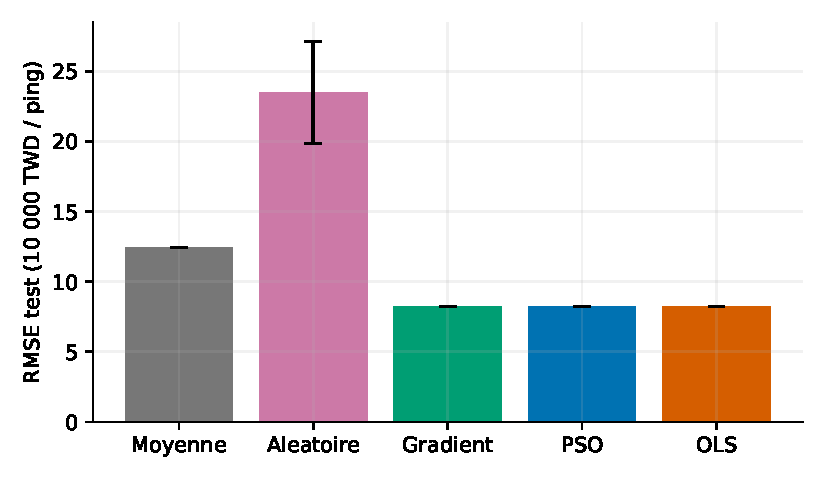
\includegraphics[width=\columnwidth]{figures/comparaison_rmse.pdf}
\caption{RMSE moyenne sur le test principal. Les barres d'erreur représentent un écart-type entre initialisations ; elles sont presque invisibles pour le PSO et nulles pour les méthodes déterministes.}\label{fig:rmse}
\end{figure}
La figure~\ref{fig:rmse} permet de comparer les ordres de grandeur. OLS, gradient et PSO ne sont pas trois modèles prédictifs différents : ce sont trois façons d'ajuster la même régression. Leur accord est donc attendu lorsque chacun réduit correctement le même objectif.

Les temps du tableau montrent que le PSO demande plus de calcul que les moindres carrés dans notre code. Pour cette régression de petite dimension, OLS est la méthode naturelle. L'intérêt du PSO est ici d'étudier une méthode sans gradient et de vérifier son comportement par une référence connue.

\subsection{Convergence et rôle de la mémoire}
La figure~\ref{fig:budget} compare les meilleurs coûts au cours des évaluations. Nous traçons l'écart avec le coût OLS plutôt que le coût brut : cela rend visibles les progrès près du minimum. L'axe vertical est logarithmique et les valeurs inférieures à $10^{-14}$ sont affichées à ce seuil pour éviter le logarithme de zéro.
\begin{figure*}[t]\centering
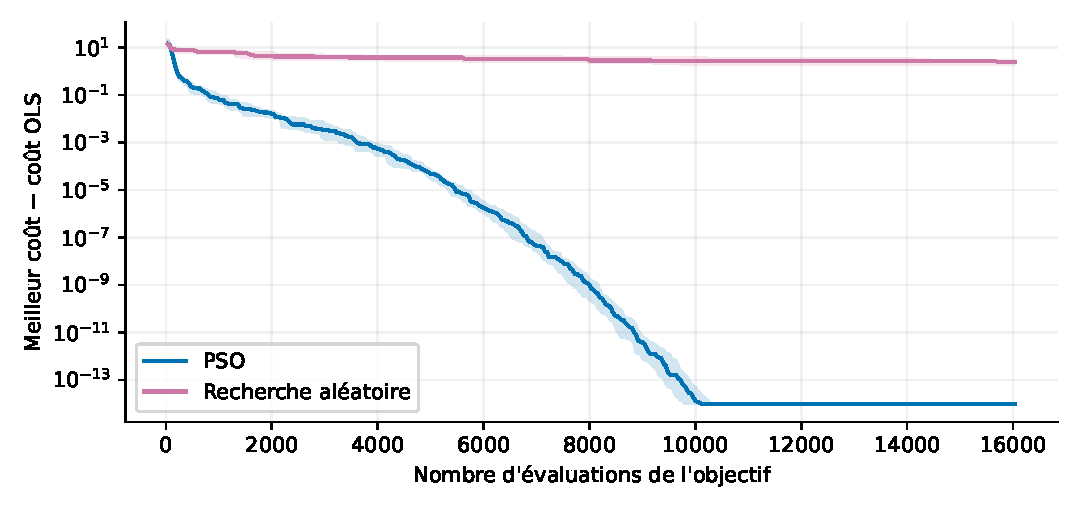
\includegraphics[width=.88\textwidth]{figures/convergence_budget.pdf}
\caption{Écart au coût OLS en fonction des évaluations : médiane de 20 graines et bande entre premier et troisième quartiles. PSO et recherche aléatoire utilisent le même budget de 16\,040 évaluations. Le seuil d'affichage est $10^{-14}$.}\label{fig:budget}
\end{figure*}
La recherche aléatoire s'améliore seulement quand un nouveau tirage dépasse le précédent. Le PSO utilise les bonnes positions déjà trouvées pour orienter les déplacements suivants. La courbe illustre l'utilité de cette mémoire sur ce problème. L'amélioration peut ralentir lorsque l'essaim se rapproche du minimum.

Le coût OLS de l'apprentissage vaut environ 0,41523734 dans l'échelle standardisée. Le PSO le retrouve à la précision numérique près. Un petit écart négatif dû aux arrondis machine n'est pas une amélioration théorique du minimum. Le code et les figures emploient une tolérance adaptée à cette précision.
\begin{figure}[t]\centering
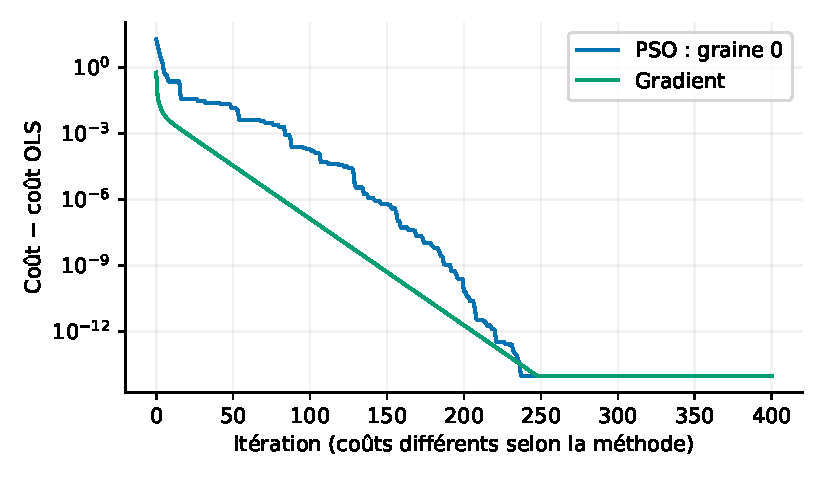
\includegraphics[width=\columnwidth]{figures/convergence_gradient.pdf}
\caption{Gradient et PSO de graine 0 : écart au coût OLS par itération. Une itération de PSO traite 40 particules ; une itération de gradient effectue une mise à jour. Ce graphique ne compare pas des budgets égaux.}\label{fig:gradient}
\end{figure}
La figure~\ref{fig:gradient} montre une autre voie vers le même minimum : la direction est calculée avec les dérivées. Elle rappelle qu'une courbe de convergence doit toujours être accompagnée de la définition de son axe horizontal. Une descente rapide par itération ne signifie pas automatiquement un meilleur temps total.

\subsection{Prédictions et résidus}
La figure~\ref{fig:predictions} représente les prédictions de la graine 0. Cette graine est utilisée comme exemple fixe, sans sélectionner celle qui donne la meilleure RMSE. La ligne en pointillés correspond à une prédiction exacte.
\begin{figure*}[t]\centering
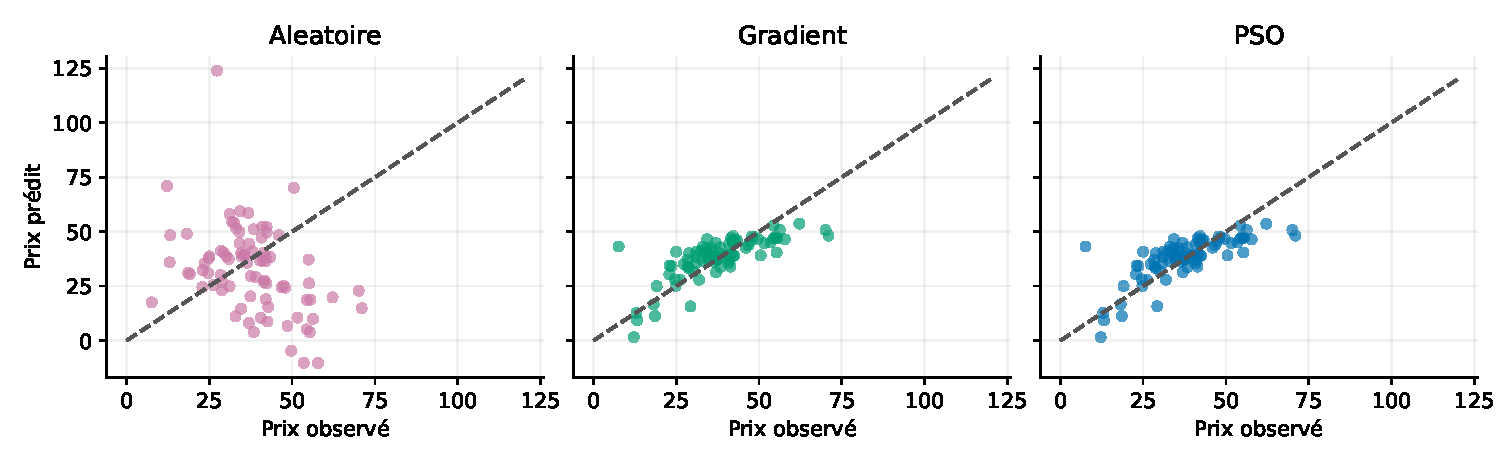
\includegraphics[width=.98\textwidth]{figures/predictions_comparees.pdf}
\caption{Prix observés et prédits sur les mêmes 83 logements : recherche aléatoire, gradient et PSO. Les deux axes sont en $10^4$ TWD par ping. Les mêmes limites d'axes facilitent la comparaison.}\label{fig:predictions}
\end{figure*}
Les nuages du gradient et du PSO se ressemblent car les coefficients sont très proches. Certaines observations restent loin de la diagonale. Le modèle linéaire ne retrouve donc pas chaque prix avec précision, même lorsque l'optimisation est quasiment exacte.

Les résidus sont définis comme le prix observé moins le prix prédit. Un résidu positif signifie une sous-estimation. Un résidu négatif signifie une surestimation. La figure~\ref{fig:residus} montre les résidus du PSO de graine 0 ainsi que leur distribution.
\begin{figure*}[t]\centering
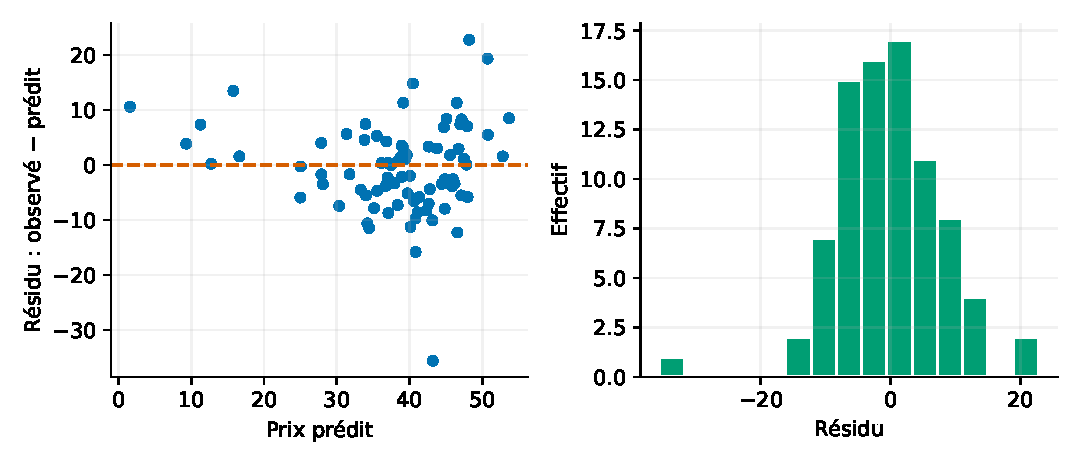
\includegraphics[width=.88\textwidth]{figures/residus.pdf}
\caption{Résidus du PSO, graine 0, sur le test principal. Prix et résidus sont en $10^4$ TWD par ping. La ligne orange représente une erreur nulle. Aucun point n'a été retiré.}\label{fig:residus}
\end{figure*}
L'histogramme ne suffit pas pour établir que les erreurs suivent une loi normale. De même, une absence de motif évident dans le nuage ne prouve pas l'absence de biais. Cette analyse sert à repérer les grandes erreurs et les limites de la forme linéaire ; elle ne remplace pas un diagnostic statistique complet.

\subsection{Stabilité entre initialisations}
La figure~\ref{fig:stabilite} trace la RMSE de chaque initialisation pour le PSO et la recherche aléatoire. Les lignes de référence correspondent à OLS. Les échelles verticales sont différentes : le panneau PSO montre surtout des différences d'arrondi de très faible amplitude, alors que la recherche aléatoire présente des écarts réels entre graines.
\begin{figure*}[t]\centering
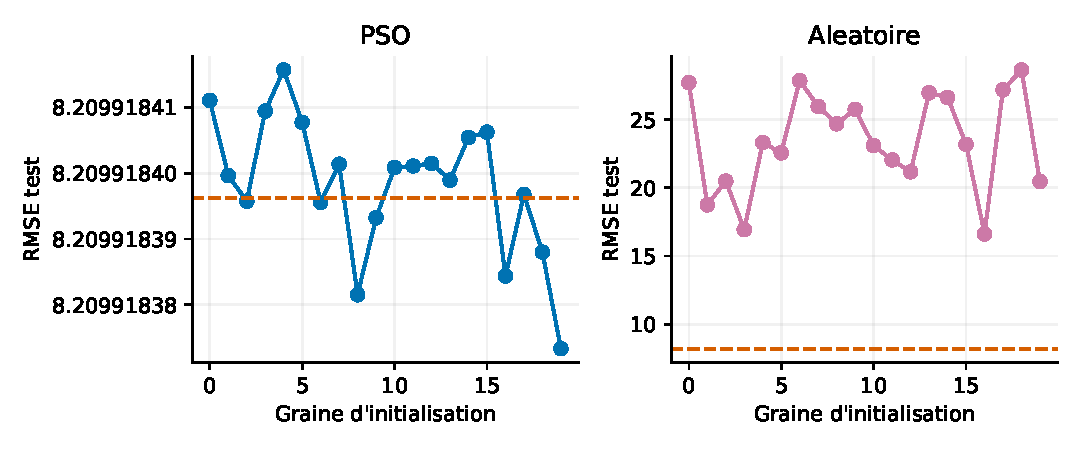
\includegraphics[width=.88\textwidth]{figures/stabilite.pdf}
\caption{Vingt graines sur le même partage. Chaque panneau possède sa propre échelle verticale. Les variations très faibles du PSO ne doivent pas être interprétées comme une incertitude immobilière négligeable.}\label{fig:stabilite}
\end{figure*}
Le PSO est stable dans ce protocole, mais ce résultat concerne uniquement la recherche des coefficients. Tous les essais utilisent le même test. Ils ne représentent pas vingt nouvelles bases indépendantes. Il serait incorrect de calculer à partir de cette seule dispersion un intervalle de confiance pour le prix d'un logement.

\subsection{Taille de l'essaim à budget court}
Pour observer l'effet du nombre de particules avant une convergence complète, nous fixons un budget court de 1\,600 évaluations, initialisation comprise. Les tailles 10, 20, 40 et 80 correspondent respectivement à 159, 79, 39 et 19 itérations. Chaque configuration est exécutée avec les graines 0 à 9.
\begin{figure}[t]\centering
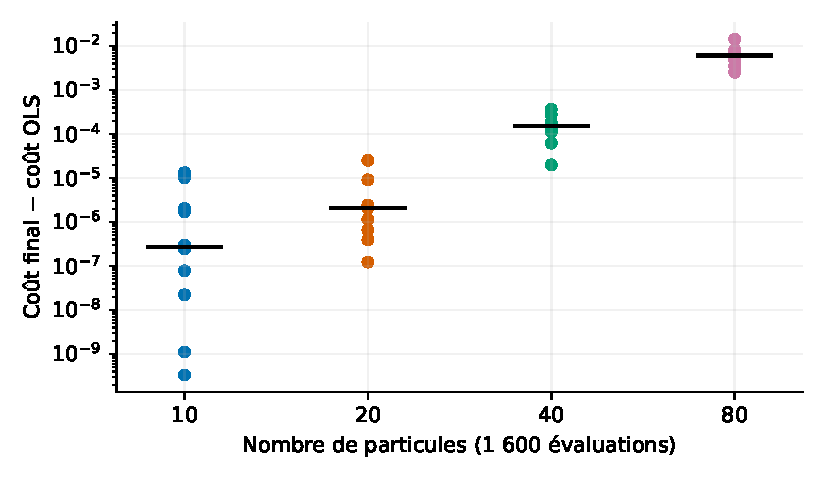
\includegraphics[width=\columnwidth]{figures/sensibilite.pdf}
\caption{Sensibilité à la taille de l'essaim : écart final au coût OLS pour dix graines, budget de 1\,600 évaluations. Les points sont les exécutions et le trait noir leur médiane. Aucun score de test n'est utilisé.}\label{fig:sensibilite}
\end{figure}
À budget égal, un grand essaim dispose de davantage de positions simultanées mais de moins de déplacements successifs. Un petit essaim explore moins de positions à la fois, mais peut les améliorer pendant plus d'itérations. La figure~\ref{fig:sensibilite} permet d'observer ce compromis sans modifier le modèle final selon le test.

Cette expérience ne définit pas une taille optimale universelle. Elle se limite à sept coefficients et à ce budget. Avec le budget long de l'expérience principale, les différences finales peuvent devenir très faibles. La sensibilité est donc surtout informative sur les étapes intermédiaires de l'optimisation.

\subsection{Variation selon les logements de test}
Nous répétons le partage 80/20 avec les graines 10, 20, 30, 40 et 50, fixées comme expériences complémentaires. À chaque fois, les moyennes et écarts-types sont recalculés sur le nouvel apprentissage. Le PSO utilise la graine 0 et ses paramètres principaux. Nous conservons tous les résultats, sans ne rapporter que le meilleur.
\begin{table}[t]\centering\small
\caption{Autres partages : RMSE du PSO de graine 0 et d'OLS, sans sélection du meilleur partage.}
\label{tab:partages}
\begin{tabular}{lrr}\toprule
Graine du partage & PSO & OLS\\\midrule
10 & 8,1395 & 8,1395\\
20 & 7,3918 & 7,3918\\
30 & 11,2513 & 11,2513\\
40 & 7,6446 & 7,6446\\
50 & 7,3337 & 7,3337\\
\bottomrule
\end{tabular}
\end{table}

\begin{figure}[t]\centering
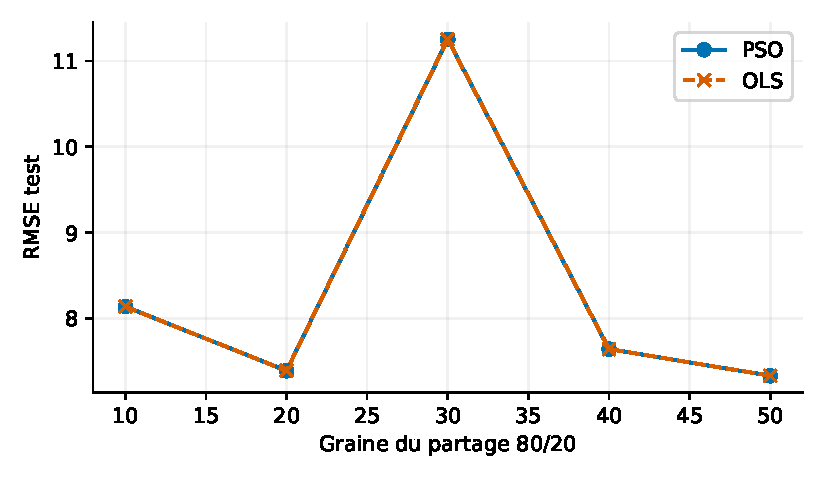
\includegraphics[width=\columnwidth]{figures/partages.pdf}
\caption{RMSE sur cinq autres partages : les courbes PSO et OLS se superposent pratiquement. Les tests peuvent partager des lignes entre expériences ; ils ne sont pas indépendants.}\label{fig:partages}
\end{figure}
Le tableau~\ref{tab:partages} et la figure~\ref{fig:partages} montrent une variation plus importante que celle due aux initialisations du PSO. La RMSE varie ici d'environ 7,33 à 11,25. La difficulté des logements présents dans le test influence donc fortement le score. Le fait que PSO et OLS restent proches indique que cette variation ne vient pas principalement d'un échec du PSO.

Nous ne présentons pas ces cinq partages comme une validation croisée indépendante ou un test statistique de supériorité. Les ensembles se recouvrent et la base reste petite. L'expérience sert à montrer la fragilité d'une conclusion construite sur un seul partage aléatoire.

\subsection{Lecture des coefficients}
La figure~\ref{fig:coefficients} compare les coefficients standardisés du PSO de graine 0 et d'OLS sur le partage principal. Leur accord complète la comparaison des prédictions et du coût. La standardisation facilite la comparaison des échelles des coefficients.
\begin{figure}[t]\centering
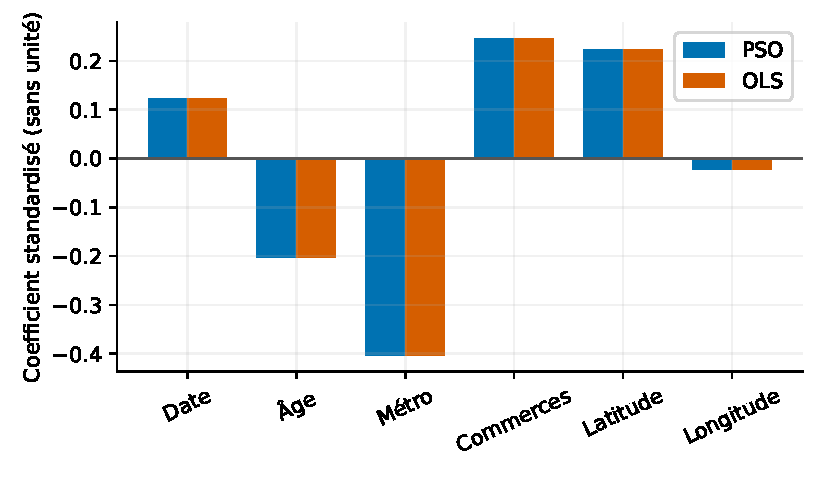
\includegraphics[width=\columnwidth]{figures/coefficients.pdf}
\caption{Coefficients standardisés des six variables, hors constante. Les poids PSO et OLS sont presque identiques. Le signe indique un lien conditionnel dans le modèle, pas un effet causal.}\label{fig:coefficients}
\end{figure}
Un coefficient négatif signifie que la prédiction diminue avec cette variable lorsque les autres restent fixes. Cette lecture doit rester prudente : latitude, longitude et distance décrivent en partie la même organisation spatiale. Le poids d'une variable ne représente donc pas une importance unique, indépendante des autres colonnes.

\section{Application, code et reproductibilité}
\subsection{Organisation des fichiers}
Le projet comporte une version courte et une étude complémentaire. Le fichier \texttt{experience.py} permet de suivre la préparation, le PSO et la comparaison OLS. Le fichier \texttt{etude\_complete.py} ajoute les deux autres optimiseurs, les répétitions et les figures de cet article. Les fonctions utilisent des boucles explicites et des noms en français. Aucun service d'intelligence artificielle externe n'est appelé pendant les calculs.

Les calculs utilisent NumPy \cite{numpy} et les figures utilisent Matplotlib \cite{matplotlib}. Les PDF vectoriels conservent la lisibilité et les couleurs distinguent les méthodes.

Les CSV conservent les scores, les durées et les expériences par graine. Un JSON réunit les résumés et alimente les tables de l'article. L'Excel original et sa provenance sont inclus.
\subsection{Fonctionnement de l'interface}
L'application contient six champs correspondant exactement aux variables de la base. Elle lit la constante et les six coefficients déjà calculés, puis effectue une somme de produits. Elle n'entraîne pas le modèle à chaque clic et ne propose pas un prix total.

Le résultat est affiché en $10^4$ TWD par ping et converti à titre indicatif en TWD par m$^2$ avec l'approximation UCI. La ville et la période sont affichées pour éviter une utilisation comme estimation actuelle. Une combinaison dans les bornes des champs peut rester peu représentée dans la base.
\subsection{Contrôles effectués}
Les contrôles portent sur l'identité numérique entre l'Excel et le CSV, la séparation des lignes du partage principal, la monotonie du meilleur coût, l'absence de prédictions non finies et l'accord avec OLS à la tolérance numérique. La transformation inverse des coefficients est aussi vérifiée contre les prédictions standardisées.

Le test fonctionnel de l'interface vérifie le chargement des six champs et deux saisies suivies d'un calcul. Cela ne garantit pas l'absence d'erreur sur toutes les machines. Le fichier de dépendances et les commandes de lancement permettent de refaire les essais dans un environnement Python compatible.

\section{Limites de l'étude}
\subsection{Validité des données et du modèle}
Le nombre d'observations est limité. Les données portent sur une seule zone et sur une période ancienne. Les scores ne peuvent pas être transférés aux prix actuels, à une autre ville ou au Maroc. La base ne décrit pas toutes les informations utiles, comme l'état intérieur ou la surface totale.

La relation linéaire peut être insuffisante pour les effets de localisation. Nous avons conservé ce modèle pour rester dans le sujet du module. Ajouter des réseaux de neurones ou des arbres sans protocole clair ne rendrait pas automatiquement l'étude plus scientifique. Une extension devrait d'abord préciser la question et la façon d'évaluer un modèle plus complexe.
\subsection{Limites de l'évaluation}
Les partages aléatoires peuvent placer des logements voisins dans l'apprentissage et le test. Ils mesurent donc une interpolation dans la base plus qu'une prédiction géographique nouvelle. Une évaluation par zone ou par date serait nécessaire pour des conclusions plus larges.

Nous ne réglons pas de nouveaux hyperparamètres sur le test. L'étude de taille d'essaim examine seulement le coût d'apprentissage et ne choisit pas un nouveau modèle final. Pour une recherche systématique de meilleurs réglages, il faudrait ajouter une validation interne puis conserver un test final non consulté pendant les décisions.

Les temps sont mesurés avec des implémentations simples. Une version vectorisée du PSO pourrait être plus rapide. Les résultats de durée montrent le coût du code fourni et ne démontrent pas une propriété générale de complexité pratique. Les répétitions déterministes ne créent pas de nouveaux échantillons statistiques.

\section{Conclusion et perspectives}
Cette étude compare plusieurs façons d'ajuster une même régression linéaire sur 414 observations réelles. Le PSO retrouve une solution proche des moindres carrés et du gradient. Il dépasse la recherche aléatoire uniforme au même budget d'évaluations dans le domaine choisi. En revanche, il ne donne pas de gain prédictif établi sur OLS et demande plus de calcul dans notre implémentation.

Les expériences répétées montrent une distinction essentielle : le PSO peut être très stable alors que le score varie sensiblement selon les logements retenus pour le test. Les graphiques de prédiction et de résidus rappellent aussi qu'un minimum numérique précis n'élimine pas les limites du modèle.

Les suites utiles seraient une base plus récente, un partage temporel ou géographique, une validation pour les réglages et, ensuite, une comparaison contrôlée avec un modèle non linéaire. Le présent travail constitue une étude reproductible d'optimisation, avec des données et des résultats explicitement documentés.

\begin{thebibliography}{00}
\bibitem{kennedy} J. Kennedy and R. Eberhart, ``Particle swarm optimization,'' in \textit{Proc. ICNN}, vol. 4, 1995, pp. 1942--1948, doi: 10.1109/ICNN.1995.488968.
\bibitem{uci} I.-C. Yeh, \textit{Real Estate Valuation}, UCI Machine Learning Repository, 2018, doi: 10.24432/C5J30W. Licence CC BY 4.0.
\bibitem{yeh} I.-C. Yeh and T.-K. Hsu, ``Building real estate valuation models with comparative approach through case-based reasoning,'' \textit{Applied Soft Computing}, vol. 65, pp. 260--271, 2018, doi: 10.1016/j.asoc.2018.01.029.
\bibitem{shi} Y. Shi and R. Eberhart, ``A modified particle swarm optimizer,'' in \textit{Proc. IEEE Int. Conf. Evolutionary Computation}, 1998, pp. 69--73, doi: 10.1109/ICEC.1998.699146.
\bibitem{boyd} S. Boyd and L. Vandenberghe, \textit{Convex Optimization}. Cambridge University Press, 2004. [En ligne]. Disponible : \url{https://web.stanford.edu/~boyd/cvxbook/}.
\bibitem{bergstra} J. Bergstra and Y. Bengio, ``Random search for hyper-parameter optimization,'' \textit{Journal of Machine Learning Research}, vol. 13, pp. 281--305, 2012. \url{https://www.jmlr.org/papers/v13/bergstra12a.html}.
\bibitem{lstsq} NumPy, ``numpy.linalg.lstsq,'' documentation officielle. Consultée le 24 octobre 2026. \url{https://numpy.org/doc/stable/reference/generated/numpy.linalg.lstsq.html}.
\bibitem{r2} Scikit-learn, ``r2\_score,'' documentation officielle. Consultée le 24 octobre 2026. \url{https://scikit-learn.org/stable/modules/generated/sklearn.metrics.r2_score.html}.
\bibitem{numpy} C. R. Harris \textit{et al.}, ``Array programming with NumPy,'' \textit{Nature}, vol. 585, pp. 357--362, 2020, doi: 10.1038/s41586-020-2649-2.
\bibitem{matplotlib} J. D. Hunter, ``Matplotlib: A 2D graphics environment,'' \textit{Computing in Science \& Engineering}, vol. 9, no. 3, pp. 90--95, 2007, doi: 10.1109/MCSE.2007.55.
\end{thebibliography}
\end{document}
